\documentclass[../main]{subfiles}

\begin{document}

\section{Functions and Linear Graphs}

\subsection{Cartesian Coordinates}

The \textbf{Cartesian coordinate system} describes the positions of points and
lines in a plane. A Cartesian plane consists of a horizontal axis and a vertical
axis.
\begin{enumerate}
\item The horizontal axis: \textbf{x-axis}
\item  The vertical axis: \textbf{y-axis}
\item The two axes intersect at the origin, \(O\).

\end{enumerate}

The position of any point on the Cartesian plane is represented as an ordered
pair \((a,b)\) of real numbers know as \textbf{coordinates}.

Note:
\(a\) is know as the \(x-coordinate\)

\(b\) is know as the \(y-coordinate\)

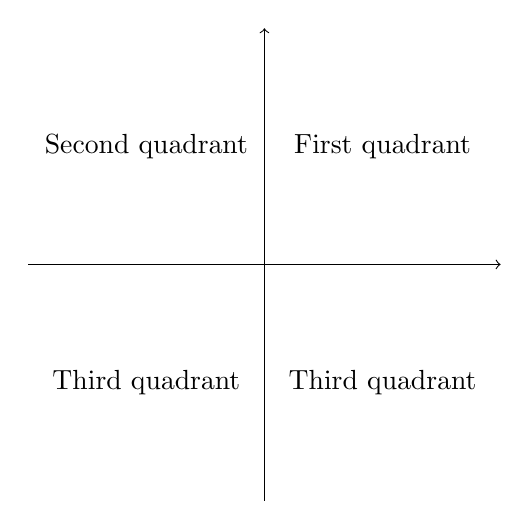
\begin{tikzpicture}[scale=1.5]
  \coordinate (0) at (0,0);
  \draw [->] (-2, 0 ) -- (2,0);
  \draw [<-] (0,2) -- (0,-2) ;
  \node at (1,1) []{First quadrant};
  \node at (-1,1) []{Second quadrant};
  \node at (-1,-1) []{Third quadrant};
  \node at (1,-1) []{Third quadrant};

\end{tikzpicture}

The position of any point on the Cartesian plane is represented as an ordered
pair(a,b) of real numbers known as \textbf{coordinates}.

\begin{tikzpicture}
  \draw [->]  (-2,0) -- (2, 0) ;
  \draw [<-] (0,2) -- (0, -2);
  \draw [densely dotted] (1, 0) -- (1,1) -- (0, 1);
  \node at (1,0)[below] {$a$};
  \node at (0,1)[left] {$b$};
  \node at (2,0) [right] {$x$};
  \node at (0,2)[above] {$y$};
  \node at (0,0)[left,below] {$O$};
  \node at (1,1)[circle,fill=black]{};
\end{tikzpicture}

Notes:
\begin{itemize}
\item \(a\) is known as the \(x-\)coordinate.
\item \(b\) is known as the \(y-\)coordinate.
\item the coordinate of the origin is \((0,0)\).
\end{itemize}
  
\subsection{Functions}
The relationship between two variables can be investigated by plotting a graph
on a Cartesian plane.

A \textbf(linear graph) is a graph in the form of a straight line.

The equation of a linear graph is of the form \(y=mx +c\), where \(m\) and \(c\)
are constants. \(x\) and \(y\) are the two variables where their relationship is
to be investigated.
\begin{enumerate}
\item  The graphs of equations of the form \(y=a\) or \(x =a\) where $a$ is a
  constant are also \textbf{linear}.
 
\item The graph of \(y=a\) is a straight \textbf{horizontal} line where \(x=a\)
  is a straight \textbf{vertical} line.
\end{enumerate}

\subsection{Graphs of linear functions}
Steps in plotting a linear graph:
\begin{enumerate}[label=(\alph*)]
\item From the information given, construct a table for the values of $x$ and
  $y$ (if the table is not given).
 
\item On a sheet of graph paper, 
  \begin{enumerate}[label=(\roman*)]
  \item draw and label the $x$-axis and $y$-axis,
  \item plot the points using the values from the table in (a)
  \item join the points to form a straight line. 
  \end{enumerate}
\end{enumerate}
\item Label the graph with the equation of the line.

Note: Pay attention on the information given in the question. Sometimes, the
variable(s) used for the $x$-axis and/or $y$-axis not $x$ and/or $y$.

\subsection{Gradient of a straight line}

The \textbf{gradient} or \textbf{slope} of a straight line is the measure of the
steepness of the line. It is defined as follows:
\[{Gradient\ of\ \ \ line}={\frac {vertical\ change} {horizontal\ change}}\]

The \textbf{greater} the numerical value of a gradient, the \textbf{steeper} the line.


  
\end{document}